% \begin{itemize}
%     \item \textbf{Question:}
%     \item \textbf{Answer:}
% \end{itemize}
\section{Exercise 1}\label{sec:exercises}
One is provided with 2 files, 1 per sattelite. Each file contains 5 columns, from left to right those columns contain the following data:
\begin{enumerate}
    \item the time in seconds from an arbitrary start point 0.
    \item the latitude of the pixel on the ground in (micro, you need to divide by million ) degrees
    \item the longitude of the pixel on the ground in (micro, you need to divide by million ) degrees
    \item The ssh = sea surface height in an unspecified unit.
    \item unknown?
\end{enumerate}

\subsection{Exercise 1A}
Make a scatter plot of track 1 vs track 2.

To do this, one would like to see whether, if the altitude in track one goes up, whether the altitude in track 2 also goes up. The first way coming to mind on how to connect these was:
\begin{enumerate}
    \item by looking at the measurements of the same position $i$, and then plotting a dot at (x=ssh track 1 on pos $i$, y = ssh track 2 on pos $i$). 
    \item To determine whether there are measurements taken on the same position the dataset is inspected. Unfortunatly the lattitude slightly varies between the two making it not possible.
    \item A different approach would be to use time as their unifying property, but that also differs.
    \item Another approach is to use their element index as unifying property. That works but is limited to 156 elements, as that is the length of the shortest dataset (found in track 2).
\end{enumerate}
Hence as a solution, the ssh of track 1 is contains the x coordinate of the scatterplot of the 156 dots, and the ssh of track 2 contains the y coordinates of the scatterplot of the 156 dots.

\subsubsection*{Matlab code}
\newpage
\lstinputlisting{code/Exercise1a.m}

\begin{itemize}
    \item \textbf{Question:}What would be the meaning of a scatterplot in the form of an x? Would it mean there is mostlikely an extra dimension that would cause the 2nd/other trend (1 line is large positive covariance, the other line is large negative covariance).
    \item \textbf{Answer:}
\end{itemize}
\subsubsection{Matlab plots:}
Some plot
\begin{figure}[h!]
    \centering
    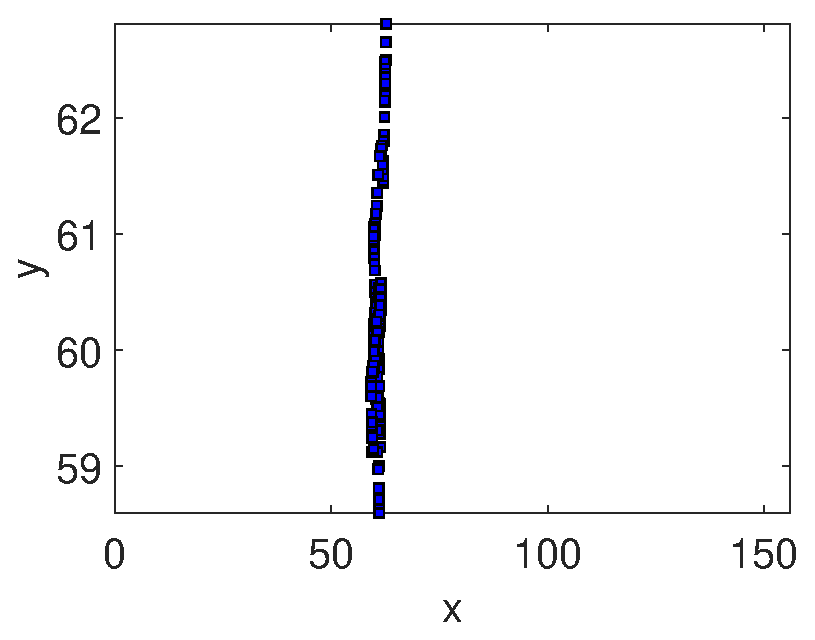
\includegraphics{images/matlabEx1/verticalLine}
    \caption{If you set the axis domain it will automatically turn it into a vertical line.}
    \label{fig:vertical_line}
\end{figure}
\begin{figure}[h!]
    \centering
    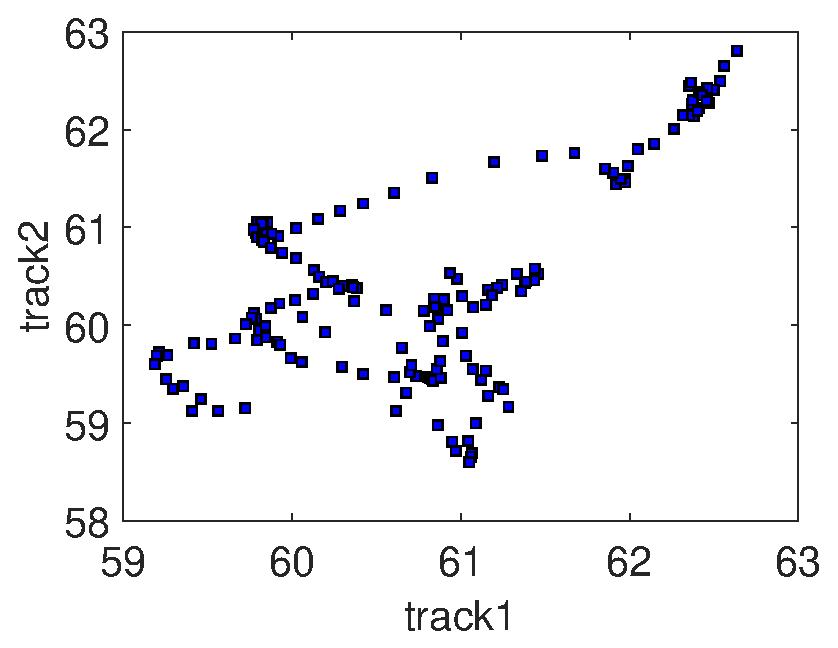
\includegraphics{images/matlabEx1/scatterplot.eps}
    \caption{Correct scatterplot.}
    \label{fig:vertical_line}
\end{figure}
\begin{figure}[h!]
    \centering
    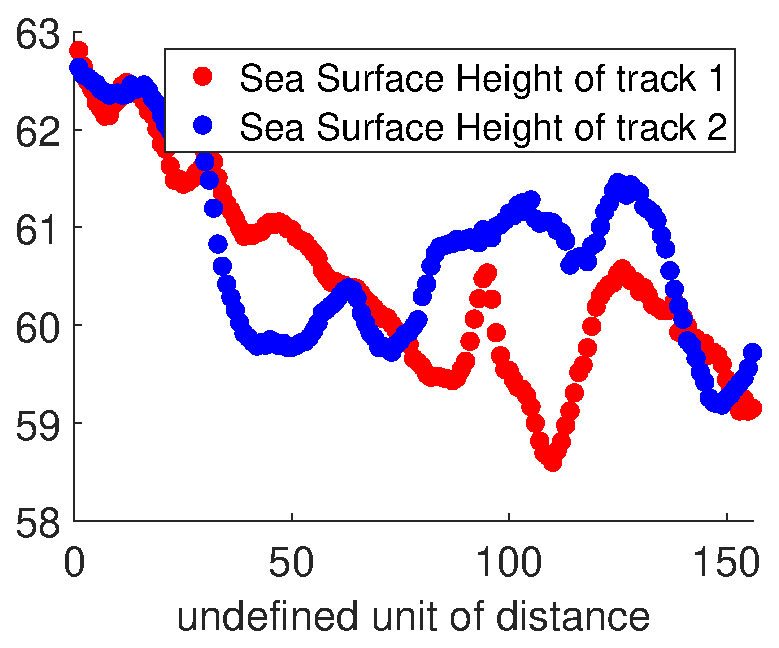
\includegraphics{images/matlabEx1/twoTimeSeries}
    \caption{Two timeseries.}
    \label{fig:vertical_line}
\end{figure}

\begin{itemize}
    \item \textbf{Question:} Why does matlab turn the scatterplot into a vertical line if the axis domains are automatically defined?
    \item \textbf{Answer:}
\end{itemize}

\newpage
\subsection{Exercise 1b}
To compute the covariance, normally one would use a density function of the data. For example, suppose you have a lolly with chewinggum in the core, you could write a function/express of the density as a function of the radius. This could be a symbolic, continuous integratable density function (Those are the PDF's {Probability Density Functions} in lecture 1 pdf slide 14/51). However in real life you often don't know the density of your dataset is, imagine an fMRI of people going to MacDonalds in such a scanner on a damped trolly because they have to lie still for it to scan accurrately, you do not know how dense their brain activity regarding a certain topic might be, hence if you want to determine the covariance of their associations with fries with certain landmarks whilst going to MacDonalds in an fMRI scanner, you might want to assume the density of their associations based on the datapoints along the way to MacDonals, instead of dertermining the exact symbolic function that describes their density.

Therefore, lecture slide 26/51 computes the covariance matrix of 2 dataseries as:
\begin{equation}
P=E
\begin{bmatrix}
    {(X-E(X))}^2       & (X-E(X))(Y-E(Y))\\
    (X-E(X))(Y-E(Y)    & {(Y-E(Y))}^2\\
    % \hdotsfor{5} \\
\end{bmatrix}    
\label{eq:covariance_with_expected_value}
\end{equation}
Where:

\begin{enumerate}
    \item $E(X)$ is the expected value of $XE$, which is the mean of $X$.
\end{enumerate}

\begin{itemize}
    \item \textbf{Question:} What does the expected value $E$ (in front of matrix) of that matrix, mean? /What is the difference between \cref{eq:covariance_with_expected_value} and \cref{eq:covariance_without_expected_value}?
    \begin{equation}
P=
\begin{bmatrix}
    {(X-E(X))}^2       & (X-E(X))(Y-E(Y))\\
    (X-E(X))(Y-E(Y)    & {(Y-E(Y))}^2\\
    % \hdotsfor{5} \\
\end{bmatrix}    
\label{eq:covariance_without_expected_value}
\end{equation}
    \item \textbf{Answer:} Lecture 1 pdf slide 25/51 states E(X) is a function of $X$: ${\int_{-\infty}}^{\infty}x\cdot f(x)dx$ where the $f(x)$ is a gaussian probability distribution. Since you probably still don't know that gaussian probability distribution, you have to find a numerical way.
\end{itemize}

So this can also be written as:
\begin{equation}
P=E
\begin{bmatrix}
    {\sigma}^2(X)       & \mu_{12}\\
    \mu_{12}    & {\sigma}^2(X)\\
    % \hdotsfor{5} \\
\end{bmatrix}    
\end{equation}
Where $\sigma$ is the standard deviation, which in Matlab can be computed with std(X), and $\mu$ is computed as the mean of the two data series.

But in matlab the formula is:
\begin{equation}
    P_{yy} = \frac{1}{n}\cdot \sum_{i=0}^{n-1}{(x_i-\mu_x)\cdot (y_i-\mu_y)}
\end{equation}

This yields:
\newpage
\lstinputlisting{code/Exercise1b.m}



\begin{itemize}
    \item \textbf{Question:} ?
    \item \textbf{Answer:}
\end{itemize}



\begin{itemize}
    \item \textbf{Question:} ?
    \item \textbf{Answer:}
\end{itemize}